\begin{figure}[!htbp]
\begin{center}

\begin{subfigure}[b]{\linewidth}
\begin{minipage}{\linewidth}
\centering
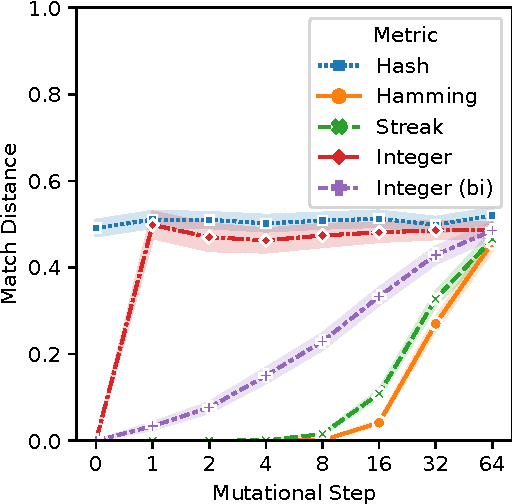
\includegraphics[width=0.75\linewidth]{img/mutational_walk/bitweight=0dot5+seed=1+title=mutational_walk_lineplot_ci+_data_hathash_hash=8bf152d87daa9cb7+_script_fullcat_hash=44400a7961ad5f3b+ext=}

\end{minipage}
\begin{minipage}{\linewidth}
\caption{
Mean match distances along mutational walks.
Error bands represent bootstrapped 95\% confidence intervals.
Note logarithmic scale on the $x$ axis.
}
\end{minipage}
\end{subfigure}

\begin{subfigure}[b]{\linewidth}
\begin{minipage}{\linewidth}
\centering
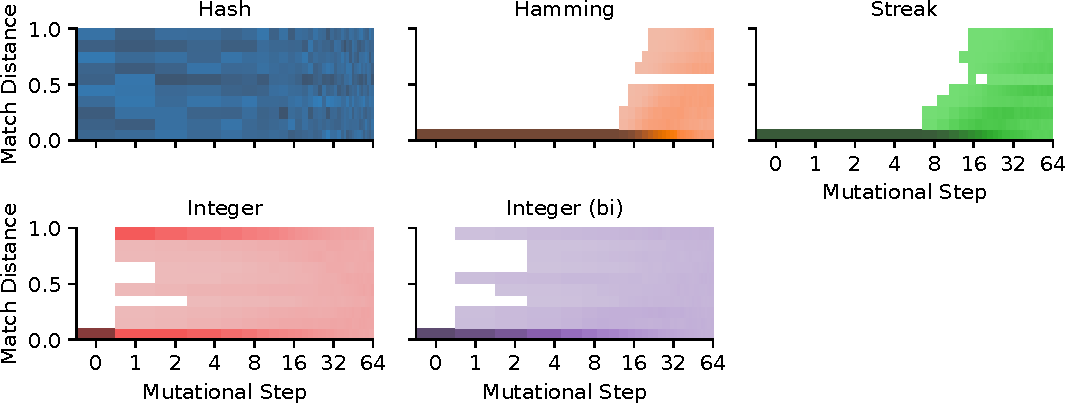
\includegraphics[width=\linewidth]{img/mutational_walk/bitweight=0dot5+seed=1+title=mutational_walk_heatplot+_data_hathash_hash=8bf152d87daa9cb7+_script_fullcat_hash=3e4b97b1d7992e5a+ext=}

\end{minipage}
\begin{minipage}{\linewidth}
\caption{
Distribution of match distances along mutational walks.
Note logarithmic scale on the $x$ axis.
}
\end{minipage}
\end{subfigure}

\caption{
Match distance along 5,000 sampled mutational walks from initially identical tags.
Note that, unlike other metrics where tags always exhibit 0.0 self-match distance (i.e., at mutational step 0), the hash metric exhibits arbitrary self-match distance by construction (see Section \ref{sec:hash}).
}
\label{fig:mutational_walk_barplot}

\end{center}
\end{figure}
